\documentclass[12pt,a4paper]{article}
\usepackage[utf8]{inputenc}
\usepackage{amsmath,amsfonts,amssymb}
\usepackage{graphicx}
\usepackage{hyperref}
\usepackage{geometry}
\usepackage{tabularx}
\usepackage{booktabs}
\usepackage{tikz}
\usetikzlibrary{positioning, arrows.meta, calc, decorations.pathreplacing, fit}
\usepackage{float}
\usepackage{fancyhdr}
\usepackage{xcolor}
\usepackage{listings}

\geometry{margin=1in}
\pagestyle{fancy}
\fancyhf{}
\rhead{Meowcessor - Register File Documentation}
\lhead{\today}
\cfoot{\thepage}

\definecolor{codegreen}{rgb}{0,0.6,0}
\definecolor{codegray}{rgb}{0.5,0.5,0.5}
\definecolor{codepurple}{rgb}{0.58,0,0.82}
\definecolor{backcolour}{rgb}{0.95,0.95,0.92}

\lstdefinestyle{mystyle}{
    backgroundcolor=\color{backcolour},   
    commentstyle=\color{codegreen},
    keywordstyle=\color{magenta},
    numberstyle=\tiny\color{codegray},
    stringstyle=\color{codepurple},
    basicstyle=\ttfamily\footnotesize,
    breakatwhitespace=false,         
    breaklines=true,                 
    captionpos=b,                    
    keepspaces=true,                 
    numbers=left,                    
    numbersep=5pt,                  
    showspaces=false,                
    showstringspaces=false,
    showtabs=false,                  
    tabsize=2
}
\lstset{style=mystyle}

\begin{document}

\title{\textbf{Meowcessor CPU Project}\\ \Large Register File \& ALU Datapath Integration Design Document}
\author{Aadi}
\date{\today}
\maketitle

\tableofcontents
\newpage

% ============================================================================
\section{Introduction}
% ============================================================================

This document details the architecture, implementation, and verification of the \textbf{Register File} for the Meowcessor RISC-V 32-bit CPU, as well as its integration with the previously completed ALU wrapper. The register file is the CPU's fastest and most frequently accessed storage, providing operands to the ALU and receiving computation results on every instruction cycle.

The RISC-V RV32I base integer instruction set specifies 32 general-purpose registers, each 32 bits wide, with register \texttt{x0} permanently hardwired to zero. Our implementation adheres to this specification exactly.

% ============================================================================
\section{What Is a Register File?}
% ============================================================================

\subsection{The Memory Hierarchy Analogy}

A CPU interacts with multiple levels of storage, each trading capacity for speed:

\begin{enumerate}
    \item \textbf{Registers} — The fastest storage. A tiny scratchpad (32 slots in RISC-V) built directly inside the CPU core from flip-flops. Access is effectively instantaneous (combinational read, single-cycle write).
    \item \textbf{Cache (L1/L2/L3)} — Small but fast SRAM close to the CPU. Access takes a few cycles.
    \item \textbf{Main Memory (RAM)} — Large but slower DRAM. Access takes tens to hundreds of cycles.
    \item \textbf{Storage (SSD/HDD)} — Massive capacity but very slow. Access takes millions of cycles.
\end{enumerate}

The register file sits at the very top of this hierarchy. Every arithmetic, logic, and data-movement instruction reads its operands from registers and writes its result back to a register.

\subsection{How a Single Register Holds a Value}

At the transistor level, a register is built from \textbf{D flip-flops} — circuits that capture and hold a single bit of data:

\begin{enumerate}
    \item Two cross-coupled inverters form a \textbf{stable feedback loop}. Once a bit enters the loop, it reinforces itself indefinitely — this is the fundamental mechanism of digital memory.
    \item A \textbf{clock-gated input} (the ``door'') controls \emph{when} new data can enter the loop. The door only opens on the \textbf{rising edge} of the clock signal and is shut at all other times.
    \item A \textbf{write-enable} signal acts as a second lock. Even if the clock edge arrives, the flip-flop only accepts new data when write-enable is asserted.
\end{enumerate}

One 32-bit register is simply \textbf{32 D flip-flops side by side}, all sharing the same clock and write-enable. On a rising clock edge with write-enable high, all 32 flip-flops simultaneously swallow their respective input bit and hold it until the next enabled clock edge.

\begin{figure}[H]
    \centering
    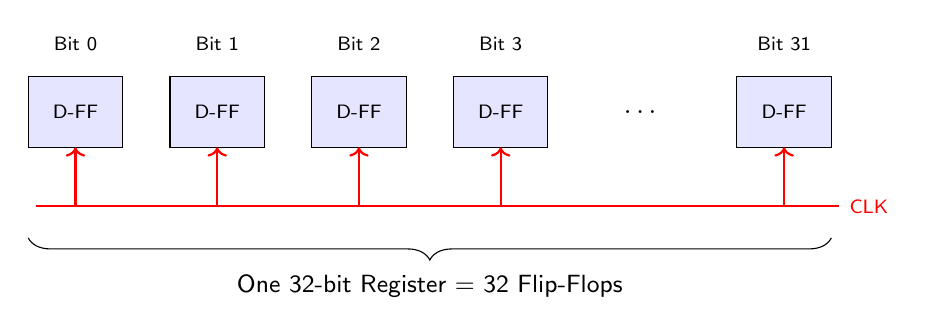
\begin{tikzpicture}[
        ff/.style={draw, rectangle, minimum width=1.2cm, minimum height=0.9cm, text centered, font=\sffamily\scriptsize, fill=blue!10},
        arrow/.style={thick,->,>=stealth}
    ]
        \foreach \i in {0,1,2,3} {
            \node (ff\i) [ff] at (\i*1.8, 0) {D-FF};
            \node [above=2mm of ff\i, font=\sffamily\scriptsize] {Bit \i};
        }
        \node (dots) at (4*1.8, 0) {\ldots};
        \node (ff31) [ff] at (5*1.8, 0) {D-FF};
        \node [above=2mm of ff31, font=\sffamily\scriptsize] {Bit 31};
        
        % Clock line
        \draw [thick, red] (-0.5, -1.2) -- (5*1.8+0.7, -1.2) node[right, font=\sffamily\scriptsize] {CLK};
        \foreach \i in {0,1,2,3} {
            \draw [thick, red, ->] (\i*1.8, -1.2) -- (\i*1.8, -0.45);
        }
        \draw [thick, red, ->] (5*1.8, -1.2) -- (5*1.8, -0.45);
        
        % Brace
        \draw [decorate, decoration={brace, amplitude=8pt, mirror}] (-0.6, -1.6) -- (5*1.8+0.6, -1.6) node[midway, below=10pt, font=\sffamily\small] {One 32-bit Register = 32 Flip-Flops};
    \end{tikzpicture}
    \caption{Structure of a single 32-bit register}
\end{figure}

% ============================================================================
\section{Architecture}
% ============================================================================

\subsection{Specification Summary}

\begin{table}[H]
    \centering
    \begin{tabularx}{\textwidth}{@{} l X @{}}
        \toprule
        \textbf{Parameter} & \textbf{Value} \\
        \midrule
        Register Count & 32 ($x_0$ through $x_{31}$) \\
        Register Width & 32 bits (parameterised as \texttt{WIDTH}) \\
        Address Width & 5 bits ($\lceil\log_2 32\rceil = 5$) \\
        Read Ports & 2 (asynchronous / combinational) \\
        Write Port & 1 (synchronous, rising edge of \texttt{clk}) \\
        Reset & Active-low asynchronous (\texttt{rst\_n}) \\
        $x_0$ Behaviour & Hardwired to \texttt{32'h0000\_0000}; writes ignored \\
        Write-Through Bypass & Enabled (same-cycle forwarding) \\
        Total Flip-Flops & $32 \times 32 = 1{,}024$ \\
        \bottomrule
    \end{tabularx}
    \caption{Register File Specifications}
\end{table}

\subsection{Port Interface}

\begin{table}[H]
    \centering
    \begin{tabularx}{\textwidth}{@{} l c c X @{}}
        \toprule
        \textbf{Signal} & \textbf{Direction} & \textbf{Width} & \textbf{Description} \\
        \midrule
        \texttt{clk}    & Input  & 1  & System clock \\
        \texttt{rst\_n} & Input  & 1  & Active-low asynchronous reset \\
        \texttt{we}     & Input  & 1  & Write enable (active high) \\
        \texttt{waddr}  & Input  & 5  & Write address (destination register $rd$) \\
        \texttt{wdata}  & Input  & 32 & Write data \\
        \texttt{raddr1} & Input  & 5  & Read address for port 1 ($rs1$) \\
        \texttt{rdata1} & Output & 32 & Read data from port 1 \\
        \texttt{raddr2} & Input  & 5  & Read address for port 2 ($rs2$) \\
        \texttt{rdata2} & Output & 32 & Read data from port 2 \\
        \bottomrule
    \end{tabularx}
    \caption{Register File Port Map}
\end{table}

\subsection{Block Diagram}

\begin{figure}[H]
    \centering
    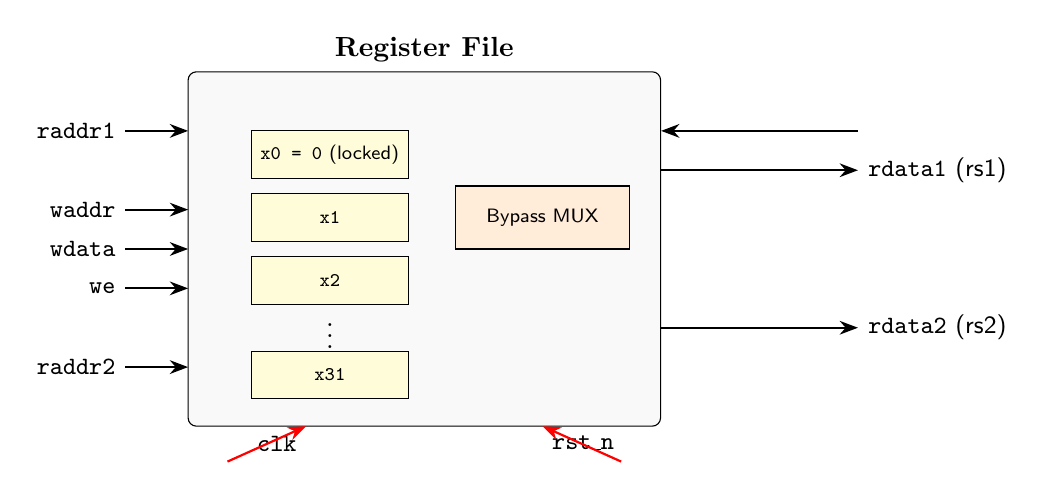
\begin{tikzpicture}[
        box/.style={draw, rectangle, minimum width=3.5cm, minimum height=1cm, text centered, font=\sffamily\small, fill=blue!10},
        regbox/.style={draw, rectangle, minimum width=6cm, minimum height=4.5cm, text centered, font=\sffamily\small, fill=gray!5, rounded corners=3pt},
        smallbox/.style={draw, rectangle, minimum width=2cm, minimum height=0.6cm, text centered, font=\sffamily\scriptsize, fill=yellow!15},
        arrow/.style={thick,->,>=Stealth}
    ]
        % Main register file box
        \node (rf) [regbox] at (0, 0) {};
        \node [above] at (rf.north) {\textbf{Register File}};
        
        % Internal registers
        \node (x0)  [smallbox] at (-1.2, 1.2) {\texttt{x0 = 0} (locked)};
        \node (x1)  [smallbox] at (-1.2, 0.4) {\texttt{x1}};
        \node (x2)  [smallbox] at (-1.2, -0.4) {\texttt{x2}};
        \node (dots) at (-1.2, -1.0) {\vdots};
        \node (x31) [smallbox] at (-1.2, -1.6) {\texttt{x31}};
        
        % Bypass MUX
        \node (byp) [box, fill=orange!15, minimum width=2.2cm, minimum height=0.8cm] at (1.5, 0.4) {\scriptsize Bypass MUX};
        
        % Read ports (outputs)
        \draw [arrow] (rf.east) ++(0, 1.0) -- ++(2.5, 0) node[right, font=\sffamily\small] {\texttt{rdata1} (rs1)};
        \draw [arrow] (rf.east) ++(0, -1.0) -- ++(2.5, 0) node[right, font=\sffamily\small] {\texttt{rdata2} (rs2)};
        
        % Read address inputs
        \draw [arrow] (rf.east) ++(2.5, 1.5) -- ++(-2.5, 0) node[left, xshift=-2.5cm, font=\sffamily\small] {};
        \node [left, font=\sffamily\small] at (-3.8, 1.5) {\texttt{raddr1}};
        \draw [arrow] (-3.8, 1.5) -- (-3, 1.5);
        
        \node [left, font=\sffamily\small] at (-3.8, -1.5) {\texttt{raddr2}};
        \draw [arrow] (-3.8, -1.5) -- (-3, -1.5);
        
        % Write port inputs
        \node [left, font=\sffamily\small] at (-3.8, 0.5) {\texttt{waddr}};
        \draw [arrow] (-3.8, 0.5) -- (-3, 0.5);
        
        \node [left, font=\sffamily\small] at (-3.8, 0.0) {\texttt{wdata}};
        \draw [arrow] (-3.8, 0.0) -- (-3, 0.0);
        
        \node [left, font=\sffamily\small] at (-3.8, -0.5) {\texttt{we}};
        \draw [arrow] (-3.8, -0.5) -- (-3, -0.5);
        
        % Clock and reset
        \node [below left, font=\sffamily\small] at (-1.5, -2.25) {\texttt{clk}};
        \draw [arrow, red] (-2.5, -2.7) -- (-1.5, -2.25);
        \node [below right, font=\sffamily\small] at (1.5, -2.25) {\texttt{rst\_n}};
        \draw [arrow, red] (2.5, -2.7) -- (1.5, -2.25);
        
    \end{tikzpicture}
    \caption{Register File Block Diagram}
\end{figure}

% ============================================================================
\section{Design Details}
% ============================================================================

\subsection{Hardwired Zero Register ($x_0$)}

The RISC-V specification mandates that register $x_0$ is permanently zero. Our implementation enforces this at two levels:

\begin{enumerate}
    \item \textbf{Write Protection:} The synchronous write block checks \texttt{waddr != 0} before allowing any write. If \texttt{waddr == 0}, the write is silently discarded regardless of \texttt{we}.
    \item \textbf{Read Clamping:} The combinational read logic checks \texttt{raddr == 0} and forces the output to \texttt{32'h0} without even accessing the storage array.
\end{enumerate}

\begin{lstlisting}[language=Verilog, caption={Write protection for $x_0$}]
if (we && (waddr != {ADDR_WIDTH{1'b0}})) begin
    regs[waddr] <= wdata;
end
\end{lstlisting}

This seemingly simple feature is architecturally powerful. It enables the ISA to use $x_0$ as a universal ``discard register'' (throw away unwanted results), a constant zero source (for moves, clears, and comparisons), and a NOP generator (\texttt{addi x0, x0, 0}).

\subsection{Asynchronous (Combinational) Read Ports}

Both read ports are implemented as purely combinational logic using continuous assignments. There is \textbf{no clock latency} for reads — the output data appears on \texttt{rdata1} / \texttt{rdata2} within the propagation delay of a multiplexer after \texttt{raddr1} / \texttt{raddr2} changes.

This is essential for single-cycle and pipelined CPU architectures where the decode/execute stage must receive operand values within the same clock cycle that the instruction is decoded.

\subsection{Synchronous Write Port}

Writes are captured on the \textbf{rising edge of \texttt{clk}} when \texttt{we == 1} and \texttt{waddr != 0}. This ensures that register contents change at well-defined, predictable instants — preventing glitches and metastability.

\subsection{Internal Write-Through Bypass (Forwarding)}

\subsubsection{The Problem}

Consider two back-to-back instructions:
\begin{verbatim}
    Instruction 1:   add  x4, x1, x2     // x4 = x1 + x2 = 52
    Instruction 2:   mul  x5, x4, x3     // x5 = x4 * x3
\end{verbatim}

Instruction 2 needs the value of \texttt{x4} that was \emph{just computed} by Instruction 1. However, the write to \texttt{x4} only takes effect on the rising clock edge. If Instruction 2 reads \texttt{x4} during the same cycle that Instruction 1 is writing it, it would read the \emph{old, stale} value.

\subsubsection{The Solution}

The register file detects this conflict combinationally and \textbf{bypasses} the storage array, forwarding the write data directly to the read output:

\begin{lstlisting}[language=Verilog, caption={Write-through bypass logic}]
assign rdata1 = (!rst_n || (raddr1 == {ADDR_WIDTH{1'b0}}))
                    ? {WIDTH{1'b0}} :           // Reset or x0
                (we && (waddr == raddr1))
                    ? wdata :                    // Bypass: forward fresh data
                      regs[raddr1];              // Normal: read from storage
\end{lstlisting}

The priority chain is:
\begin{enumerate}
    \item If in reset or reading $x_0$: output zero.
    \item If the read address matches the current write address and write is enabled: output the write data directly (bypass).
    \item Otherwise: output the stored register value normally.
\end{enumerate}

This adds zero latency and eliminates the need for external forwarding logic or pipeline stalls for this class of data hazard.

% ============================================================================
\section{ALU Datapath Integration}
% ============================================================================

The register file connects to the ALU to form the core execution datapath of the Meowcessor. The data flow for an R-type instruction (e.g., \texttt{add x4, x1, x2}) proceeds as follows:

\begin{figure}[H]
    \centering
    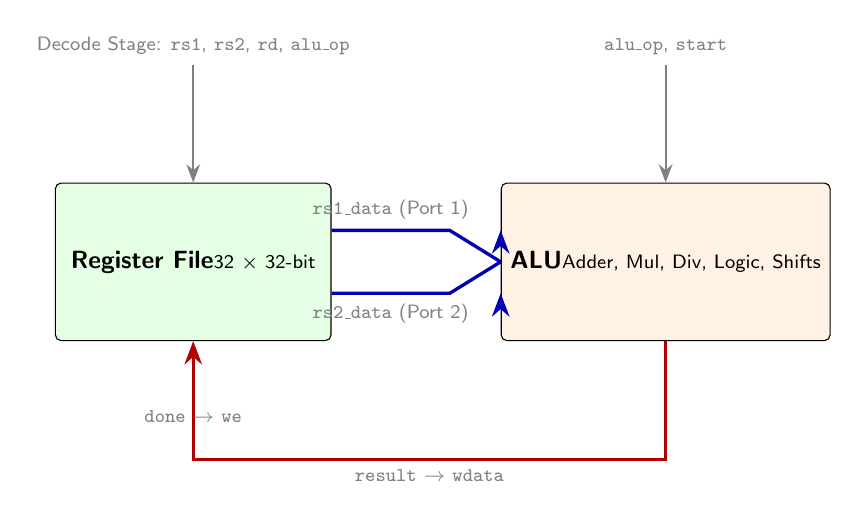
\begin{tikzpicture}[
        box/.style={draw, rectangle, minimum width=3cm, minimum height=1.2cm, text centered, font=\sffamily\small, fill=blue!10, rounded corners=2pt},
        arrow/.style={thick,->,>=Stealth},
        label/.style={font=\sffamily\scriptsize, text=gray}
    ]
        % Nodes
        \node (rf) [box, fill=green!10, minimum width=3.5cm, minimum height=2cm] at (0, 0) {\textbf{Register File}\\\scriptsize 32 $\times$ 32-bit};
        \node (alu) [box, fill=orange!10, minimum width=3.5cm, minimum height=2cm] at (6, 0) {\textbf{ALU}\\\scriptsize Adder, Mul, Div, Logic, Shifts};
        
        % Forward path: RegFile -> ALU
        \draw [arrow, blue!70!black, line width=1.2pt] (rf.east) ++(0, 0.4) -- ++(1.5, 0) node[midway, above, label] {\texttt{rs1\_data} (Port 1)} -- (alu.west) ++(0, 0.4);
        \draw [arrow, blue!70!black, line width=1.2pt] (rf.east) ++(0, -0.4) -- ++(1.5, 0) node[midway, below, label] {\texttt{rs2\_data} (Port 2)} -- (alu.west) ++(0, -0.4);
        
        % Return path: ALU -> RegFile
        \draw [arrow, red!70!black, line width=1.2pt] (alu.south) -- ++(0, -1.5) -| (rf.south) node[pos=0.25, below, label] {\texttt{result} $\rightarrow$ \texttt{wdata}} node[pos=0.75, below, label] {\texttt{done} $\rightarrow$ \texttt{we}};
        
        % Control signals from top
        \draw [arrow, gray] (0, 2.5) -- (rf.north) node[pos=0, above, label] {Decode Stage: \texttt{rs1}, \texttt{rs2}, \texttt{rd}, \texttt{alu\_op}};
        \draw [arrow, gray] (6, 2.5) -- (alu.north) node[pos=0, above, label] {\texttt{alu\_op}, \texttt{start}};
        
    \end{tikzpicture}
    \caption{Register File $\longleftrightarrow$ ALU Datapath}
\end{figure}

\subsection{Execution Sequence for a Single-Cycle Operation}

\begin{enumerate}
    \item \textbf{Operand Fetch:} The decode stage drives \texttt{raddr1 = rs1} and \texttt{raddr2 = rs2}. The register file's combinational read ports immediately output the operand values on \texttt{rdata1} and \texttt{rdata2}.
    \item \textbf{ALU Execution:} The ALU receives the operands, performs the operation selected by \texttt{alu\_op}, and produces a result within the same clock cycle (for single-cycle ops like ADD, SUB, AND, etc.).
    \item \textbf{Write-Back:} The ALU asserts \texttt{done}, which gates the register file's write enable. The result is written into \texttt{regs[rd]} on the next rising clock edge.
\end{enumerate}

\subsection{Execution Sequence for a Multi-Cycle Operation}

For operations like MUL (17 cycles) or DIV ($\sim$18 cycles):

\begin{enumerate}
    \item Steps 1 is the same as above.
    \item The ALU asserts \texttt{busy} and begins iterating internally.
    \item The register file holds the \texttt{waddr = rd} value stable while waiting.
    \item When the ALU finally asserts \texttt{done}, the result is written back to \texttt{regs[rd]} on the next rising clock edge.
\end{enumerate}

\subsection{Chained Dependency Demonstration}

The integration testbench verifies a multi-instruction dependency chain that exercises the full datapath loop repeatedly:

\begin{align*}
    x_{26} &= x_{21} + x_{22} = 5 + 15 = 20 \\
    x_{27} &= x_{26} \times x_{23} = 20 \times 8 = 160 \quad \text{(uses result of previous line)} \\
    x_{28} &= x_{27} - x_{24} = 160 - 10 = 150 \quad \text{(uses result of previous line)} \\
    x_{29} &= x_{28} \div x_{25} = 150 \div 5 = 30 \quad \text{(uses result of previous line)}
\end{align*}

Each instruction depends on the result of the instruction before it. All four instructions passed verification, confirming that the register file correctly stores and supplies intermediate values across sequential ALU operations.

% ============================================================================
\section{Synthesis Results}
% ============================================================================

The register file was synthesised using Yosys to verify correct elaboration and resource usage.

\begin{table}[H]
    \centering
    \begin{tabularx}{0.7\textwidth}{@{} l r X @{}}
        \toprule
        \textbf{Cell Type} & \textbf{Count} & \textbf{Purpose} \\
        \midrule
        \texttt{\$\_DFFE\_PN0P\_} & 1,024 & D flip-flops (32 regs $\times$ 32 bits) \\
        \texttt{\$\_AND\_}        & 2,083 & Write decode \& bypass logic \\
        \texttt{\$\_OR\_}         & 2,224 & Read mux \& bypass logic \\
        \texttt{\$\_MUX\_}        &   192 & Read port multiplexers \\
        \texttt{\$\_NOT\_}        &   114 & Inverters \\
        \texttt{\$\_XOR\_}        &    10 & Address comparison \\
        \midrule
        \textbf{Total}            & \textbf{5,647} & \\
        \bottomrule
    \end{tabularx}
    \caption{Yosys Gate-Level Cell Count for \texttt{regfile}}
\end{table}

Key observations:
\begin{itemize}
    \item Exactly \textbf{1,024 flip-flops} were inferred, confirming that all 32 registers $\times$ 32 bits are correctly mapped to sequential storage elements.
    \item \textbf{No latches} were inferred, confirming clean synchronous design with no unintended combinational feedback loops.
    \item The bypass/forwarding logic adds approximately 200 combinational cells of overhead — a negligible cost for eliminating a class of pipeline data hazards.
\end{itemize}

% ============================================================================
\section{Verification Summary}
% ============================================================================

\begin{table}[H]
    \centering
    \begin{tabularx}{\textwidth}{@{} l c X @{}}
        \toprule
        \textbf{Testbench} & \textbf{Result} & \textbf{Coverage} \\
        \midrule
        \texttt{regfile\_tb.v} & \textbf{1,165 / 1,165 PASSED} & Reset state, $x_0$ protection, full address sweep, dual-port concurrent reads, write-through bypass, 500-step randomised stress test \\
        \addlinespace
        \texttt{regfile\_alu\_tb.v} & \textbf{21 / 21 PASSED} & Register initialisation, single-cycle ALU ops (ADD, SUB, SLL, SRL, SRA, AND, OR, XOR, SLT, SLTU), multi-cycle ALU ops (MUL, DIV, REM), $x_0$ writeback protection, chained dependency pipeline \\
        \bottomrule
    \end{tabularx}
    \caption{Verification Results}
\end{table}

% ============================================================================
\section{Conclusion}
% ============================================================================

The Register File is fully implemented, synthesised, and verified. It passes all 1,186 test vectors across the standalone and integration testbenches. The module correctly implements the RISC-V RV32I register file specification with internal write-through bypass for data hazard mitigation.

Combined with the previously completed ALU, the Meowcessor now has a functional execution datapath capable of performing all RV32IM arithmetic, logic, shift, comparison, multiplication, and division operations with register-level operand sourcing and result write-back.

The next integration target is the \textbf{Instruction Decoder (ID Stage)}, which will map 32-bit RV32IM machine code into the control signals (\texttt{rs1}, \texttt{rs2}, \texttt{rd}, \texttt{alu\_op}) that drive this datapath.

\end{document}
